\section{Case Study}

The composer and recorder player Claire Farrell approached me, asking for my opinion on how to notate an extended technique that she had been developing. 
The technique involves the recorder player covering the window hole with their index finger or hand, which results in the recorder producing a whistle like effect. 
Air pressure determines the pitch, and the degree to which the window hole is covered determines the fundamental's presence or lack thereof, with full occlusion of the window producing solely the harmonic. 

This is an ideal place in which to explore the ways in which we map actions into notation; the question becomes one of how this can be achieved in the most recognisable and orderly manner. 
Our goal of establishing a defined notation system is to ensure that it is as clear and easy to understand as possible. 

Thus began an informative exploration through the various ways that we can map sound onto an instrument. 
This is an especially interesting topic to me, as I am interested in the ways in which the semiotics of notation influence its parsing. 
We can treat this development of the notation of a new technique as a case study for best practices, and establish some ground rules on how the written form of Western art music can be adapted to accomodate new techniques that fall outside of the initial set.



% \begin{itemize}
% \item Textually, through the use of just text instructions. 
% Examples would include `mute'.
% \item Textually and pictographically, with text describing complex operations, aided by the shorthand of symbols. 
% Examples would include `mute unmute'.
% 	\item Pictographically; this would encompass all techniques that are divorced from the reality of the object, such as harmonics. 
% As this is a very broad category, it can be broken down further:
% 		\item Pictographically with symbols, such as our harmonic example.
% 		\item Pictographically, with mappings to physical objects, such as the pedal sign representing the lifting of the pedal, or the half-hole representing a partially occluded hole.
% \end{itemize}

\subsection{Building from Pre-existing Notation}

Maintaining compatibility with existing Western music notation is only possible if we follow the rules that are set out in existing symbols and structures.
This means that we cannot mutate existing symbols, or ascribe a different meaning to their common one; there are to be no uses of the piano pedal symbol to indicate a patch change on an electric keyboard.
Similarly, we cannot expect the user to intuitively understand symbols that don't follow the existing design language.

We first establish that if using a pictographic notation, that there is a point at which the instrument's sound window cannot be occluded any further. 
This would, logically, follow the pre-established convention of filled in black representing `more'. 
Further more, we know that there is a point at which there is no occlusion; the exact opposite. 
However, the precise location of this point is variable.

Pictographic notation\fxnote{Explain what pictographic notation is earlier} is most useful when there are elements that cannot be conveyed succinctly with text; while it is true that one could notate it as `cover window with hand to produce high pitched seagull sound', it would be cumbersome to read and interpret quickly.\fxnote{Is it? Says who? And why do they say it? And what will the method or practice that you are talking about and demonstrating in your compositions solve this?}
Reducing that to `cover window' might result in unfortunate misinterpretations. 
Those examples\fxnote{Which examples?} also treat the act of covering the window as a binary; in discussions with the recorder player Claire Farrell, she described how the sound can change when you cover it partially, fully, or even stick your finger inside the window, blocking the free passage of air slightly to create a wholly new sound. 
So, we can safely establish that it is not feasible to use a textual direction with some degree of certainty; 
minute differences between covering the window from 30 percent to 50 percent and back to 20 percent would be unnecessarily verbose, or filled with numbers that were divorced from contextual information.\fxnote{needs a lot of refinement and consideration re place and purpose in the argument}

An aural equivalent can be drawn from double bass repertoire, in which a high harmonic on the bridge glissandos rapidly down to a lower partial, producing a `seagull' like effect. 
These are notated as regular harmonics, sometimes with `seagull effect' above the line. 
The double bass seagull effect is largely timbral though, and its efficacy of communicating the desired effect lies not in the notation, but in the unary nature of the intended resultant sound; a rapid dropping of a high pitch to a lower one. 
It is tied to a real world parallel, and is thus easily mapped onto the instrument.

Action parallels include the stopping of a horn with a hand, and covering windpipes on clarinets and flutes; see \autoref{fig:Asset10}.\fxnote{Fix ref} 
These are closer to the intended action, and indeed the recorder lowers a tone on full occlusion of the airway much like the horn. 
However, Claire noted an issue with the typical notation; the open circle, half-closed circle, and fully black circle had no relationship to the instrument. 
The half-occlusion of the circle was confusing as the window is a square, and fingering holes are round.
Claire was attempting to map a horn technique onto a recorder, with predictably confusing results. 

\begin{figure}
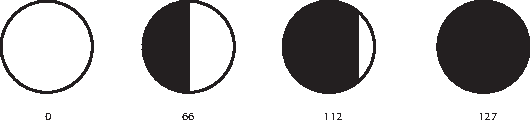
\includegraphics[width=\linewidth]{./resources/Asset10.pdf}
\caption{Half-closed circle style}\label{fig:Asset10}
\end{figure}


I modified the notation to a rectangle, to represent the rectangular window, and added black to it to represent occlusion, moving from left to right as with the half-closed circle notation; see \autoref{fig:Asset3}.
For the sake of convenience, the level of occlusion has been mapped to a MIDI rate, of 0 being totally un-occluded, with 127 being fully occluded.

\begin{figure}
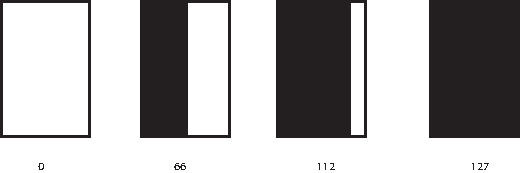
\includegraphics[width=\linewidth]{./resources/Asset3.pdf}
\caption{Modified to a rectangle}\label{fig:Asset3}
\end{figure}

However, this was obviously inappropriate, as the action of occluding the window is not a left-to-right action.
I changed it so the black increased upwards as the notation dictated further occlusion of the window as seen in \autoref{fig:Asset1}. 
This mapped similar to how a MIDI expression level is displayed as a bar graph in DAWs. 
\begin{figure}
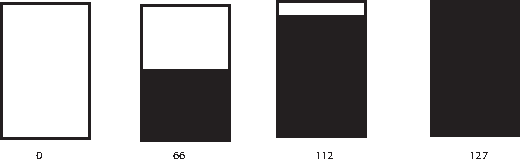
\includegraphics[width=\linewidth]{./resources/Asset1.pdf}
\caption{MIDI style range}\label{fig:Asset1}
\end{figure}

But this too posed difficulties, as the instrument's window wasn't on the bottom of the instrument, and the hand comes \emph{down} to occlude the window. 
Rotating the image 180 degrees, I found the clearest notation yet; a picture that mapped both the intended one dimensional attribute of occlusion, as well as the action onto the instrument.

\begin{figure}
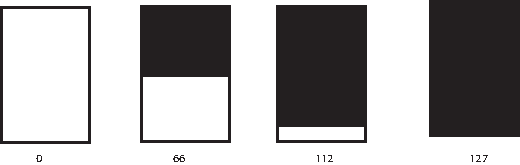
\includegraphics[width=\linewidth]{./resources/Asset2.pdf}
\caption{Inverted MIDI style range}\label{fig:Asset2}
\end{figure}

And yet, we found there was still an outlying use-case that was not accounted for; the action of pushing the finger (or, indeed, abstracted out to any object) into the window. 
This posed an interesting issue, as it challenged our one-dimensional range attribute with needing to either accommodate the inclusion of a further attribute, or a method of delineating the cutoff point for total occlusion and where the `further in' position began. 
Further compounding the issue is the fact that there is no self-evident physical point at which further insertion is impossible; 
while the occlusion has a constant point where no further occlusion is possible (i.e.\ the window is a finite opening that can be eclipsed totally), one could theoretically put objects into the window as far as physically possible.
Further attempts were made, experimenting with a perspective representation of the window to communicate a `further in' style in the single symbol; 

\begin{figure}
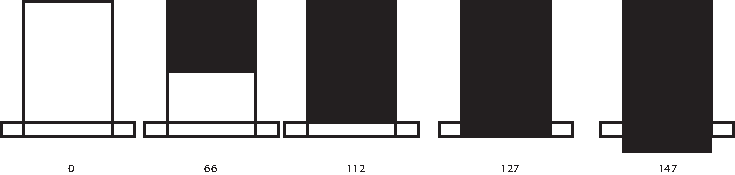
\includegraphics[width=\linewidth]{./resources/Asset4.pdf}
\caption{First attempt; without upper limit}\label{fig:Asset4}
\end{figure}

\begin{figure}
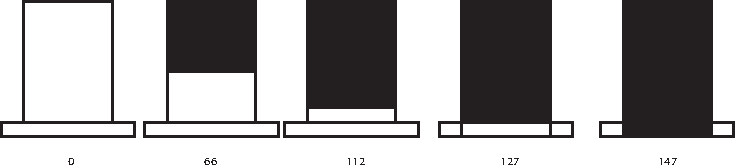
\includegraphics[width=\linewidth]{./resources/Asset5.pdf}
\caption{Second attempt; upper limit defined}\label{fig:Asset5}
\end{figure}

\begin{figure}
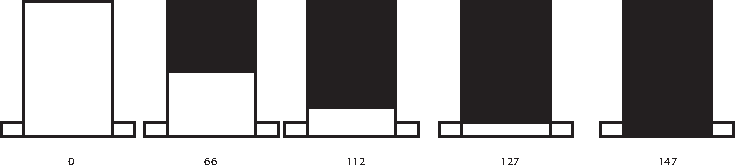
\includegraphics[width=\linewidth]{./resources/Asset6.pdf}
\caption{`Imaginary ghost finger' single perspective}\label{fig:Asset6}
\end{figure}

\begin{figure}
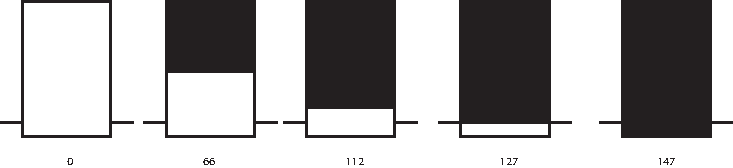
\includegraphics[width=\linewidth]{./resources/Asset7.pdf}
\caption{Side view, upper limit defined}\label{fig:Asset7}
\end{figure}

\begin{figure}
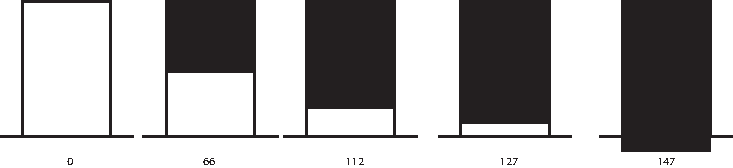
\includegraphics[width=\linewidth]{./resources/Asset9.pdf}
\caption{Side view, without upper limit}\label{fig:Asset9}
\end{figure}
